% begin module slant-asymptote-def
\begin{frame}
\frametitle{Slant Asymptotes}
\begin{definition}[Slant Asymptote]
If
\[
\lim_{x\to\infty}\left( f(x) - (mx+b)\right) = 0
\]
then the line $y = mx+b$ is called a slant asymptote for $f$.
\end{definition}
\begin{columns}[c]
\column{.4\textwidth}
\ \only<handout:0| -2>{%
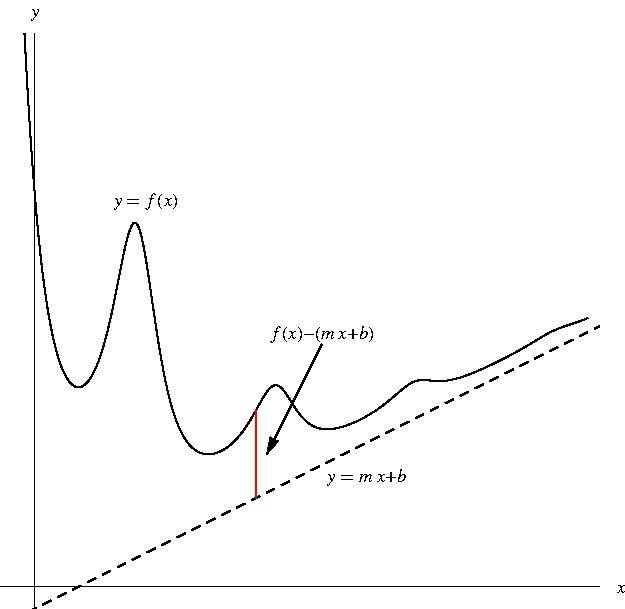
\includegraphics[width=4.5cm]{curve-sketching/pictures/04-05-slanta.pdf}%
}%
\only<handout:0| 3>{%
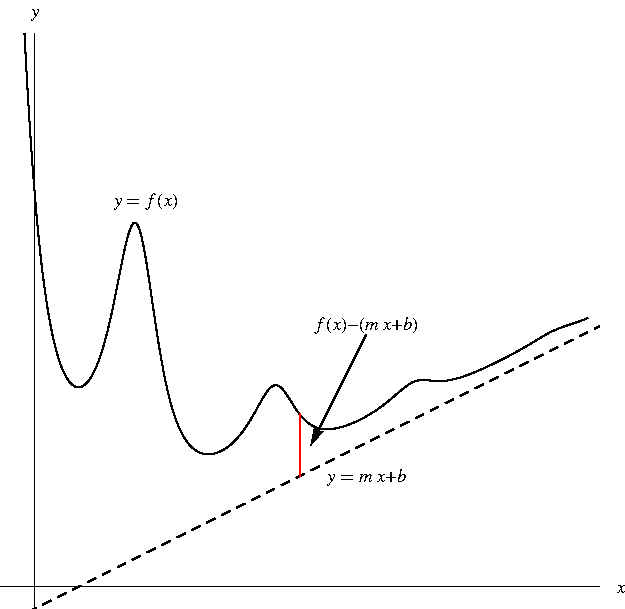
\includegraphics[width=4.5cm]{curve-sketching/pictures/04-05-slantb.pdf}%
}%
\only<handout:0| 4>{%
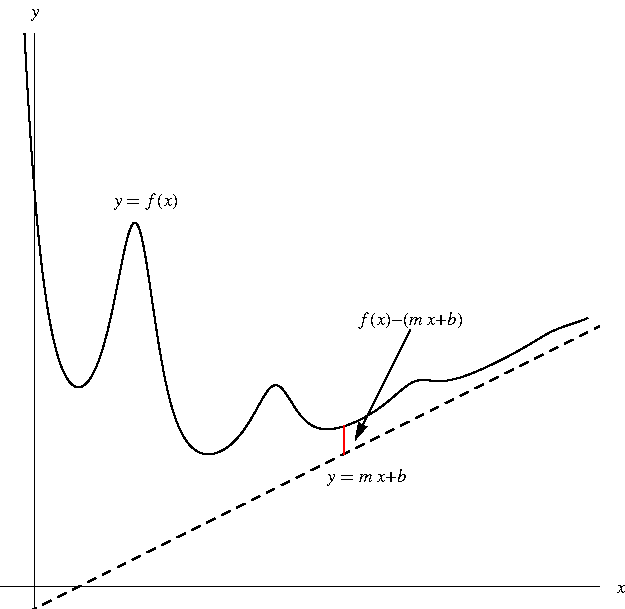
\includegraphics[width=4.5cm]{curve-sketching/pictures/04-05-slantc.pdf}%
}%
\only<5>{%
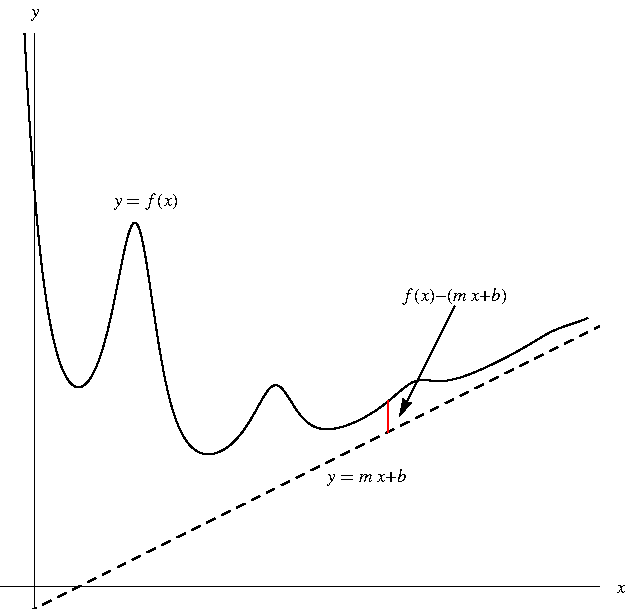
\includegraphics[width=4.5cm]{curve-sketching/pictures/04-05-slantd.pdf}%
}%
\only<handout:0| 6->{%
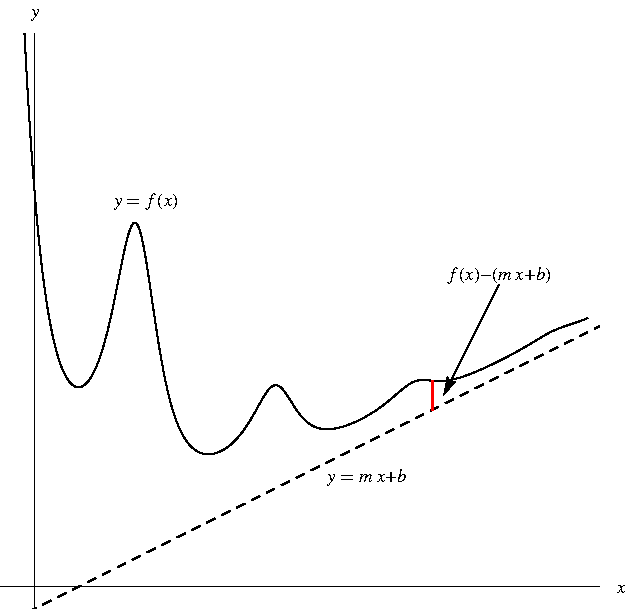
\includegraphics[width=4.5cm]{curve-sketching/pictures/04-05-slante.pdf}%
}%
\column{.6\textwidth}
\begin{itemize}
\item<2->  This means that the vertical distance between $f(x)$ and $mx+b$ approaches $0$ as $x$ gets bigger.
\item<7->  A rational function has a slant asymptote if the degree of the numerator is one more than the degree of the denominator.
\item<8->  We can find slant asymptotes using long division.
\end{itemize}
\end{columns}
\end{frame}
% end module slant-asymptote-def
